\documentclass[12pt]{article}

\documentclass[12pt]{article}

\usepackage[utf8]{inputenc}
\usepackage[english]{babel}

\usepackage{amssymb, mathtools, amsmath, amsthm}
\usepackage[italicdiff]{physics}

\usepackage[none]{hyphenat}             % disables hyphenated words at end of paragraph
%\setlength{\parindent}{0pt}             % removes paragraph indent
%\setlength{\parskip}{11pt}              % adds space between paragraphs

\usepackage{geometry}
\newlength{\alphabet}
\settowidth{\alphabet}{abcdefghijklmnopqrstuvwxyz}
\geometry{textwidth=2.5\alphabet}

\usepackage{enumitem}
\setlist[enumerate,1]{leftmargin=0pt}   % pushes enum items to the margin

%\usepackage{libertine}
%\usepackage[libertine, vvarbb]{newtxmath}

\usepackage[space]{erewhon}             % font
\usepackage[erewhon, vvarbb]{newtxmath} % math font

%\usepackage[scale=0.90]{tgheros}        % sans serif
%\usepackage[scale=0.90,lf]{FiraMono}    % monospace
\usepackage[T1]{fontenc}
\usepackage{microtype}


\newcommand{\C}{\mathbf C}
\newcommand{\F}{\mathbf F}
\newcommand{\N}{\mathbf N}
\newcommand{\PP}{\textbf P}
\newcommand{\Q}{\mathbf Q}
\newcommand{\R}{\mathbf R}
\newcommand{\Z}{\mathbf Z}

\newcommand{\inv}{^{-1}}
\newcommand{\eps}{\varepsilon}

\DeclareMathOperator{\Aut}{Aut}
\DeclareMathOperator{\Char}{char}
\DeclareMathOperator{\End}{End}
\DeclareMathOperator{\Gal}{Gal}
\DeclareMathOperator{\GL}{GL}
\DeclareMathOperator{\Hom}{Hom}
\DeclareMathOperator{\Ind}{Ind}
\DeclareMathOperator{\SL}{SL}
\DeclareMathOperator{\Spec}{Spec}

\DeclareMathOperator{\coker}{coker}
\DeclareMathOperator{\im}{im}

\newtheorem{theorem}{Theorem}
\newtheorem{lemma}[theorem]{Lemma}

\theoremstyle{definition}
\newtheorem{definition}[theorem]{Definition}

\newtheorem*{example}{Example}


\usepackage{tikz}

\title{Elementary}
\author{}
\date{}

\begin{document}

\maketitle
\tableofcontents

\newpage

\section{Trigonometry}

\subsection{The Unit Circle}

The unit circle is a circle whose radius \( r = 1 \).
We can also think of it as the set of all points \( x \) and \( y \)
such that \( x^2 + y^2 = 1 \).
By the Pythagorean Theorem,
this is also all right angle triangles whose hypotenuse is 1.

\subsubsection*{Angles in Radians}

We can measure angle in radians
by considering the ratio of arc length covered by that angle to the radius.
Thus we measure in radians the full angle of the circle as \( \frac{2\pi r}{r} = 2\pi \)
and the angle \( x \) expressed as a proportion of the full angle as \( 2\pi x \).
For example,
the angle covering \( \frac{1}{8} \) of the full angle is
\( \frac{2\pi}{8} = \frac{\pi}{4} \).

\tikzset{every picture/.style={line width=0.75pt}} %set default line width to 0.75pt        
\begin{tikzpicture}[x=0.75pt,y=0.75pt,yscale=-1,xscale=1]
%uncomment if require: \path (0,275); %set diagram left start at 0, and has height of 275

%Shape: Circle [id:dp8901582993632227] 
\draw   (21,108.5) .. controls (21,59.07) and (61.07,19) .. (110.5,19) .. controls (159.93,19) and (200,59.07) .. (200,108.5) .. controls (200,157.93) and (159.93,198) .. (110.5,198) .. controls (61.07,198) and (21,157.93) .. (21,108.5) -- cycle ;
%Straight Lines [id:da5812266179395867] 
\draw    (21,108.5) -- (200,108.5) ;
%Straight Lines [id:da3022071329689201] 
\draw    (110.5,198) -- (110.5,19) ;
%Shape: Arc [id:dp22444419057885423] 
\draw  [draw opacity=0] (121.45,99.38) .. controls (123.51,101.85) and (124.75,105.03) .. (124.75,108.5) -- (110.5,108.5) -- cycle ; \draw   (121.45,99.38) .. controls (123.51,101.85) and (124.75,105.03) .. (124.75,108.5) ;
%Straight Lines [id:da08204830136394758] 
\draw    (110.5,108.5) -- (175.5,46) ;

% Text Node
\draw (156.25,110.9) node [anchor=north west][inner sep=0.75pt]    {$r$};
% Text Node
\draw (128,93.4) node [anchor=north west][inner sep=0.75pt]    {$x$};
% Text Node
\draw (263,89.4) node [anchor=north west][inner sep=0.75pt]    {$r\ =\ 1,\ x\ =\ \frac{\pi }{4} .$};

\end{tikzpicture}

\subsection{Sine, Cosine, and Tangent}

These are functions on \( \R \),
but think of them as functions that map angles to values.
Given an angle \( x \),
we can think of each angle as specifying a right triangle.
Then, \( \cos(x) \) and \( \sin(x) \) map the angle to the sides of the triangle,
and \( \tan(x) = \frac{\sin(x)}{\cos(x)} \)
as the ratio of the two sides.

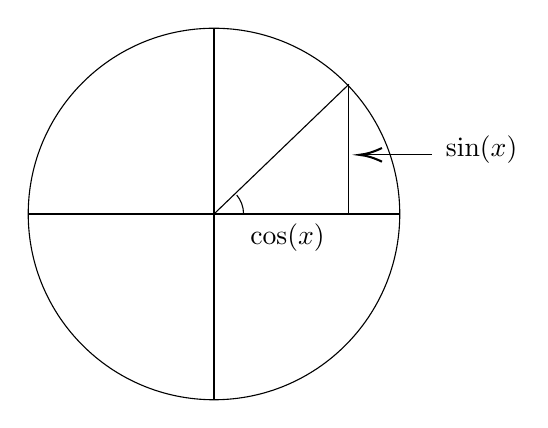
\begin{tikzpicture}[x=0.75pt,y=0.75pt,yscale=-1,xscale=1]
%uncomment if require: \path (0,300); %set diagram left start at 0, and has height of 300

%Shape: Circle [id:dp23447927429295168] 
\draw   (41,128.5) .. controls (41,79.07) and (81.07,39) .. (130.5,39) .. controls (179.93,39) and (220,79.07) .. (220,128.5) .. controls (220,177.93) and (179.93,218) .. (130.5,218) .. controls (81.07,218) and (41,177.93) .. (41,128.5) -- cycle ;
%Straight Lines [id:da45982648711254337] 
\draw    (41,128.5) -- (220,128.5) ;
%Straight Lines [id:da4472488341141133] 
\draw    (130.5,218) -- (130.5,39) ;
%Shape: Arc [id:dp8562120644249197] 
\draw  [draw opacity=0] (141.45,119.38) .. controls (143.51,121.85) and (144.75,125.03) .. (144.75,128.5) -- (130.5,128.5) -- cycle ; \draw   (141.45,119.38) .. controls (143.51,121.85) and (144.75,125.03) .. (144.75,128.5) ;
%Straight Lines [id:da5180477639280442] 
\draw    (130.5,128.5) -- (195.5,66) ;
%Straight Lines [id:da7807789607763392] 
\draw    (195.5,66) -- (195.5,129) ;
%Straight Lines [id:da737707903040607] 
\draw    (235.5,100) -- (202.5,100) ;
\draw [shift={(200.5,100)}, rotate = 360] [color={rgb, 255:red, 0; green, 0; blue, 0 }  ][line width=0.75]    (10.93,-3.29) .. controls (6.95,-1.4) and (3.31,-0.3) .. (0,0) .. controls (3.31,0.3) and (6.95,1.4) .. (10.93,3.29)   ;

% Text Node
\draw (146.75,131.9) node [anchor=north west][inner sep=0.75pt]    {$\cos( x)$};
% Text Node
\draw (241,89.4) node [anchor=north west][inner sep=0.75pt]    {$\sin( x)$};

\end{tikzpicture}

We can also look at the angle as specifying a point on the circle.
In this case,
\( (\cos(x), \sin(x)) \)
give the coordinates of the point on the circle specified by the angle
and \( \tan(x) \) is the slope of the line through that point.
In a general circle with radius \( r, \cos(x) \) and \( \sin(x) \)
give the lengths as a ratio to the radius.

\end{document}
